\chapter{相关理论与技术介绍}

\section{稀疏线性方程组求解}

经典的求解线性方程组的方法一般分为两类:直接法和迭代法。前者例如高斯消元法, LU分解等,后者的例子包括共轭梯度法等。直接法指在不考虑计算舍入误差的情况下,通过包括矩阵分解和三角方程组求解等有限步的操作求得方程组的精确解,因此又称精确法;迭代法指给定一个初始解向量,通过一定的计算构造一个向量列(一般通过逐次迭代得到一系列逼近精确值的近似解),向量列的极限为方程组理论上的精确解。

\section{稀疏矩阵的压缩方式}

存储矩阵的一般方法是采用二维数组,其优点是可以随机地访问每一个元素,因而能够容易实现矩阵的各种运算。对于稀疏矩阵,它通常具有很大的维度,有时甚大到整个矩阵(零元素)占用了绝大部分内存采用二维数组的存储方法既浪费大量的存储单元来存放零元素,又要在运算中浪费大量的时间来进行零元素的无效运算。因此必须考虑对稀疏矩阵进行压缩存储(只存储非零元素)。

\subsection{COO Format}

最简单的稀疏矩阵的存储格式称为coordinate(COO) format,这个形式只保留那些非0的值,分别使用三个数组:val, rolIdx, colIdx来对应存储数值、行号以及列号,这三个数组的大小都为矩阵非零元的个数NNZ。例如下方4x5矩阵。


$$
\begin{pmatrix}
    \label{稀疏矩阵例子}
    1 & 0 & 0 & 0 & 0 \\
    2 & 4 & 0 & 6 & 0 \\
    3 & 0 & 5 & 0 & 0 \\
    4 & 7 & 0 & 8 & 9
\end{pmatrix}
$$

~\\
~\\
~\\

该矩阵在COO存储格式下,三个数组分别为:
\begin{lstlisting}[title=COO Format]
val = {1, 2, 4, 6, 3, 5, 4, 7, 8, 9}
rolIdx = {0, 1, 1, 1, 2, 2, 3, 3, 3, 3}
colIdx = {0, 0, 1, 3, 0, 2, 0, 1, 3, 4}
\end{lstlisting}

\subsection{CSR Format}

CSR(Compressed Sparse Row)是一种按行压缩的矩阵存储形式。分别使用三个数组:val, rowPtr, colIdx来对应存储数值、行指针、以及列号。其中val和colIdx的数组大小为非零元的个数NNZ,而rowPtr数组的大小一般为m+1,其中 m 为矩阵行的个数。例如图\ref{CSR}。

\begin{figure}[htbp]
    \centering
    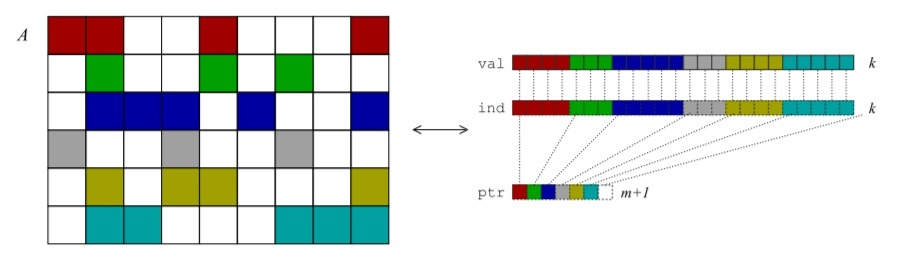
\includegraphics[width=0.7\textwidth]{CSR.png}
    \caption{CSR矩阵存储格式}
    \label{CSR}
\end{figure}

\subsection{CSC Format}

CSC(Compressed Sparse Column)与CSR相似,是一种按列压缩的矩阵存储格式。分别使用是那个数组:val, colPtr, rowIdx来对应存储数值、列指针、以及行号。其中val和rowIdx的数组大小为非零元的个数NNZ,而colPtr数组的大小一般为n+1,其中n为矩阵列的个数。例如图\ref{CSC}

\begin{figure}[htbp]
    \centering
    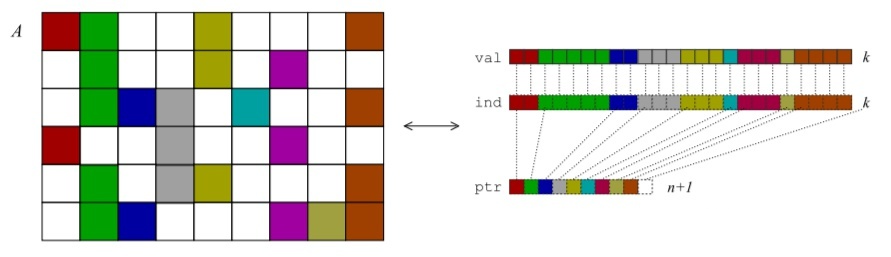
\includegraphics[width=0.7\textwidth]{CSC.png}
    \caption{CSC矩阵存储格式}
    \label{CSC}
\end{figure}

\section{已有SpTRSV算法}

\subsection{基于CSR格式的SpTRSV串行算法}

\begin{algorithm}[H]
    \caption{CSR Based Serial SpTRSV}\label{csr-serial-sptrsv}
    MALLOC(*left\_sum, n) \;
    MEMSET(*left\_sum, 0) \;
    \For{i = 0; i < n; i++}{
        \For{j = row\_ptr[i] ; j < row\_ptr[i + 1] - 1 ; j++}{
            left\_sum[i] \small{$\leftarrow$} left\_sum[i] + val[j] \small{$*$} x[col\_idx[j]] \;
         }
        x[i] \small{$\leftarrow$} (b[i] - left\_sum[i]) / val[col\_ptr[i]] \;
    }
\end{algorithm}

基于CSR格式的SpTRSV串行算法第一个循环从矩阵的第0行开始遍历这个矩阵。在第二个循环进行向量乘法的操作,求出left\_sum[i]。之后再求出未知数x[i]。

\subsection{基于CSC格式的SpTRSV串行算法}

\begin{algorithm}
    \caption{CSC Based Serial SpTRSV}\label{csc-serial-sptrsv}
    MALLOC(*left\_sum, n) \;
    MEMSET(*left\_sum, 0) \;
    \For{i = 0; i < n; i++}{
        x[i] \small{$\leftarrow$} (b[i] - left\_sum[i]) / val[col\_ptr[i]] \;
        \For{j = col\_ptr[i] + 1 ; j < col\_ptr[i + 1] ; j++}{
            left\_sum[rowIdx[j]] \small{$\leftarrow$} left\_sum[row\_idx[j]] + val[j] \small{$*$} x[i] \;
        }
    }
\end{algorithm}

该算法的第一个循环从矩阵的第0行开始遍历这个矩阵。首先求出该算该行未知数$x[i]$,接着遍历该列的上的非零元,对该列非零元所对应的$left\_sum$进行更新,$left\_sum[rowIdx[j]] += val[j] \times x[i]$。

基于CSR压缩格式SpTRSV算法以及基于CSC压缩格式的SpTRSV算法,两者在访存模式上存在着一定的差异。基于CSR格式的算法需要进行频繁离散读取未知数向量x[col\_idx[j]],相反基于CSC格式的SpTRSV算法只需要读取当前行号 i 所对应的x[i]。在写数据方面,基于CSR的并行算法需要集中的写left\_sum[i]的数据,而基于CSC的并行算法则是离散的写left\_sum[rowIdx[j]],在多核运算的条件下,离散的写比集中的写同一位置的数据更容易进行并行化。

\subsection{基于level-sets的SpTRSV并行算法}

J.Park在level-sets算法的基础上提出除了更高效的并行SpTRSV算法\cite{park2014sparsifying},该算法主要分为两个阶段:预处理阶段和计算阶段。

在预处理阶段主要有三个处理步骤:
\begin{enumerate} \setlength{\itemsep}{0pt}
\item 使用由Chhugani\cite{chhuganiFastEfficientGraph2012a}提出的高度优化的并行广度优先搜索算法(BFS),构建了一个任务依赖图\ref{TDG}。
\item 在任务依赖图的基础上,作者又通过将同level的任务合并为super-task的形式实现负载均衡,确保每个线程被分配有相似计算量的super-task,这种合并的操作有进一步减少了任务之间的依赖个数,进一步减少了同步所需的消耗。
\item 作者发现任务依赖图中存在着大量的多余依赖边,并开发了一个高效的过滤算法,去除了两条的依赖边。
\end{enumerate}

在计算阶段作者使用了与传统level-sets算法不同的调度方式,作者使用peer-to-peer的同步方式替换为了在level之间使用屏障\ref{Level-scheduling with barrier}进行同步的方式。下面是两种不同同步方式的伪代码:算法\ref{Level-scheduling with barrier}、算法\ref{Level-scheduling with peer-to-peer synchronization}

\begin{algorithm}
    \caption{Level-scheduling with barrier}
    \label{Level-scheduling with barrier}
    \ForEach{level l}{
        solve the unknowns of \small{$task_{l}^{t}$} \;
        barrier;
    }
\end{algorithm}
\begin{algorithm}
    \caption{Level-scheduling with peer-to-peer synchronization}
    \label{Level-scheduling with peer-to-peer synchronization}
    \ForEach{level l}{
        wait until all the parents are done wait \;
        solve the unknowns of \small{$task_{l}^{t}$} \;
        \textbf{done}[\small{$task_{l}^{t}$}] \;
    }
\end{algorithm}

对比两种不同的调度算法,可以发现使用peer-to-peer的调度方式,能够使得计算资源能够得到更好的利用。因为当一个线程完成任务计算之后,基于屏障的同步方式会让该线程进入等待的状态。而基于peer-to-peer的调度方式则会让该线程继续进行下去。如图\ref{两种不同同步方式的对比示意图},如果采用基于peer-to-peer的同步方式,线程2在完成任务2之后可以不用等在线程1完成任务1,可以接着运行下去。这在一定程度上也有利于负载均衡。

\begin{figure}[htbp]
    \centering
    \subfigure[通过屏障同步]{
    \begin{minipage}[t]{0.30\linewidth}
    \centering
    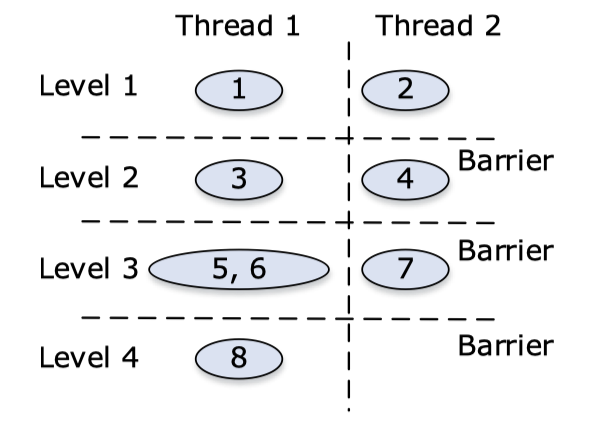
\includegraphics[height=1.3in]{sync-barrier.png}
    \end{minipage}%
    }%
    \subfigure[点对点同步]{
    \begin{minipage}[t]{0.30\linewidth}
    \centering
    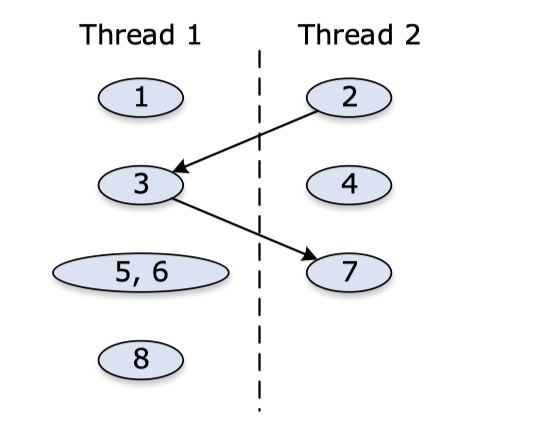
\includegraphics[height=1.3in]{sync-p2p.png}
    \label{TDG}
    \end{minipage}%
    }%
    \centering
    \caption{两种不同同步方式的对比示意图}
    \label{两种不同同步方式的对比示意图}
\end{figure}

\subsection{sync-free的SpTRSV并行算法}

\begin{table}[]
    \caption{基于level-sets算法\cite{park2014sparsifying}的任务耗时(ms)分解表}
    \label{任务耗时分解图}
    \resizebox{\textwidth}{!}{%
    \begin{tabular}{|l|l|l|l|l|l|}
    \hline
    \multirow{2}{*}{矩阵名称} &
      \multirow{2}{*}{预处理时间} &
      \multirow{2}{*}{SpTRSV计算阶段花费时间} &
      \multicolumn{2}{l|}{SpTRSV计算阶段时间分解} &
      \multirow{2}{*}{level的个数} \\ \cline{4-5}
     &
       &
       &
      同步时间消耗 &
      计算时间消耗 &
       \\ \hline
    \begin{tabular}[c]{@{}l@{}}FEM/ship 003 \\ FEM/Cantilever \\ chipcool0 \\ nlpkkt160\end{tabular} &
      \begin{tabular}[c]{@{}l@{}}92.46\\ 47.89\\ 8.74\\ 484.67\end{tabular} &
      \begin{tabular}[c]{@{}l@{}}12.95\\ 9.60\\ 1.99\\ 38.30\end{tabular} &
      \begin{tabular}[c]{@{}l@{}}10.96\\ 5.62\\ 1.15\\ 0.01\end{tabular} &
      \begin{tabular}[c]{@{}l@{}}1.99\\ 3.98\\ 0.84\\ 38.29\end{tabular} &
      \begin{tabular}[c]{@{}l@{}}4367\\ 2397\\ 534\\ 2\end{tabular} \\ \hline
    \end{tabular}%
    }
\end{table}


基于level-sets的算法需要花费大量的时间在预处理和任务间的同步上,运行J.Park的算法并分步进行统计(预处理阶段,同步所需耗时,计算阶段),我们就可以得到表\ref{任务耗时分解图}。所用的稀疏矩阵来自于佛罗里达大学的稀疏矩阵集合\cite{davis2011university},观察这张表我们可以主要得到以下几点信息:
\begin{enumerate} \setlength{\itemsep}{0pt}
\item 预处理阶段所消耗的时间,要远大于计算阶段所消耗的时间,平均大概是8至10倍左右。预处理占总时间大约80\%。
\item 同步所需的开销会导致的时间消耗,会随着矩阵level个数的增加而剧烈增加,当稀疏矩阵的level较多时,会导致同步的时间消耗远大于计算的时间消耗。这也可能是同level间负载不均衡所导致的。
\end{enumerate}

例如nlpkkt160只有两个level,同步所占用的时间要远小于计算所需的时间。作为对比矩阵FEM/ship 003,虽然矩阵的规模小于lpkkt160,但是由于其level相对较多,导致了同步所占用的时间也较多。

刘伟锋从减少预处理和减少同步所需时间的角度出发,提出了名为sync-free的SpTRSV计算方法\cite{liuSyncFree2016}。该算法能够在GPU上能够取得较好的效果。与传统基于level-sets的算法不同的是,sync-free的SpTRSV算法只在预处理阶段计算每个任务的入度,该入度表示当前任务有多少的前置依赖。作者使用一个warp,32个线程来处理每个任务。任务之间通过使用共享变量以及原子操作的方式,来决定任务之间的顺序。算法的伪代码见\ref{sync-free alogrithm preprocess}ref{sync-free alogrithm solve}

\begin{algorithm}[htbp]
    \caption{sync-free SpTRSV预处理阶段算法}
    \label{sync-free alogrithm preprocess}
    \SetKw{atomic-add}{atomic-add} 
    \SetKw{atomic-sub}{atomic-sub} 
    \SetKw{Parallel}{Parallel} 
    \SetKwProg{Fn}{Function}{ is}{end}
    malloc(*d\_left\_sum, *s\_left\_sum, *d\_in\_degree, *s\_in\_degree, n)\;
    memset(*d\_left\_sum, *s\_left\_sum, *d\_in\_degree, *s\_in\_degree, 0)\;
    \Fn{Preprocess()}{
        \Parallel \For{i = 0; i < nnz; i++}{ 
            atomic-add(\&d\_in\_degree[row\_idx[i]], 1) \; 
        }
    }
\end{algorithm}

\begin{algorithm}[htbp]
    \caption{sync-free SpTRSV计算阶段的算法}
    \label{sync-free alogrithm solve}
    \SetKw{atomic-add}{atomic-add} 
    \SetKw{atomic-sub}{atomic-sub} 
    \SetKw{Parallel}{Parallel} 
    \SetKwProg{Fn}{Function}{ is}{end}

    \Fn{Solve()}{
        \Parallel \For(using one warp for one entry){int i = 0; i < n; i++}{
            \While(test dependencies){s\_in\_degree[i] + 1 \small$\neq$ d\_in\_degree[i]}{
                // busy wait \;
            }
            \small{$x[i] \leftarrow (b[i]-d\_left\_sum[i] - s\_left\_sum[i])/val[col ptr[i]]$}\;
            \Parallel \For(one thread for one nonzero){j in \small{$[col\_ptr[i]+1], col\_ptr[i+1]-1$}}{
                \uIf{in local}{
                    atomic-add(\&s\_left\_sum[rid], \small{$val[j] \times x[i]$}) \;
                    atomic-add(\&s\_in\_degree[rid], 1) \;
                }
                \Else{
                    atomic-add(\&s\_left\_sum[rid], \small{$val[j] \times x[i]$}) \;
                    atomic-add(\&s\_in\_degree[rid], 1) \;
                }
            }

        }

    }
    
\end{algorithm}

\section{基于缓存的优化技术}

\subsection{内存cache}

\begin{figure}[htbp]
    \centering
    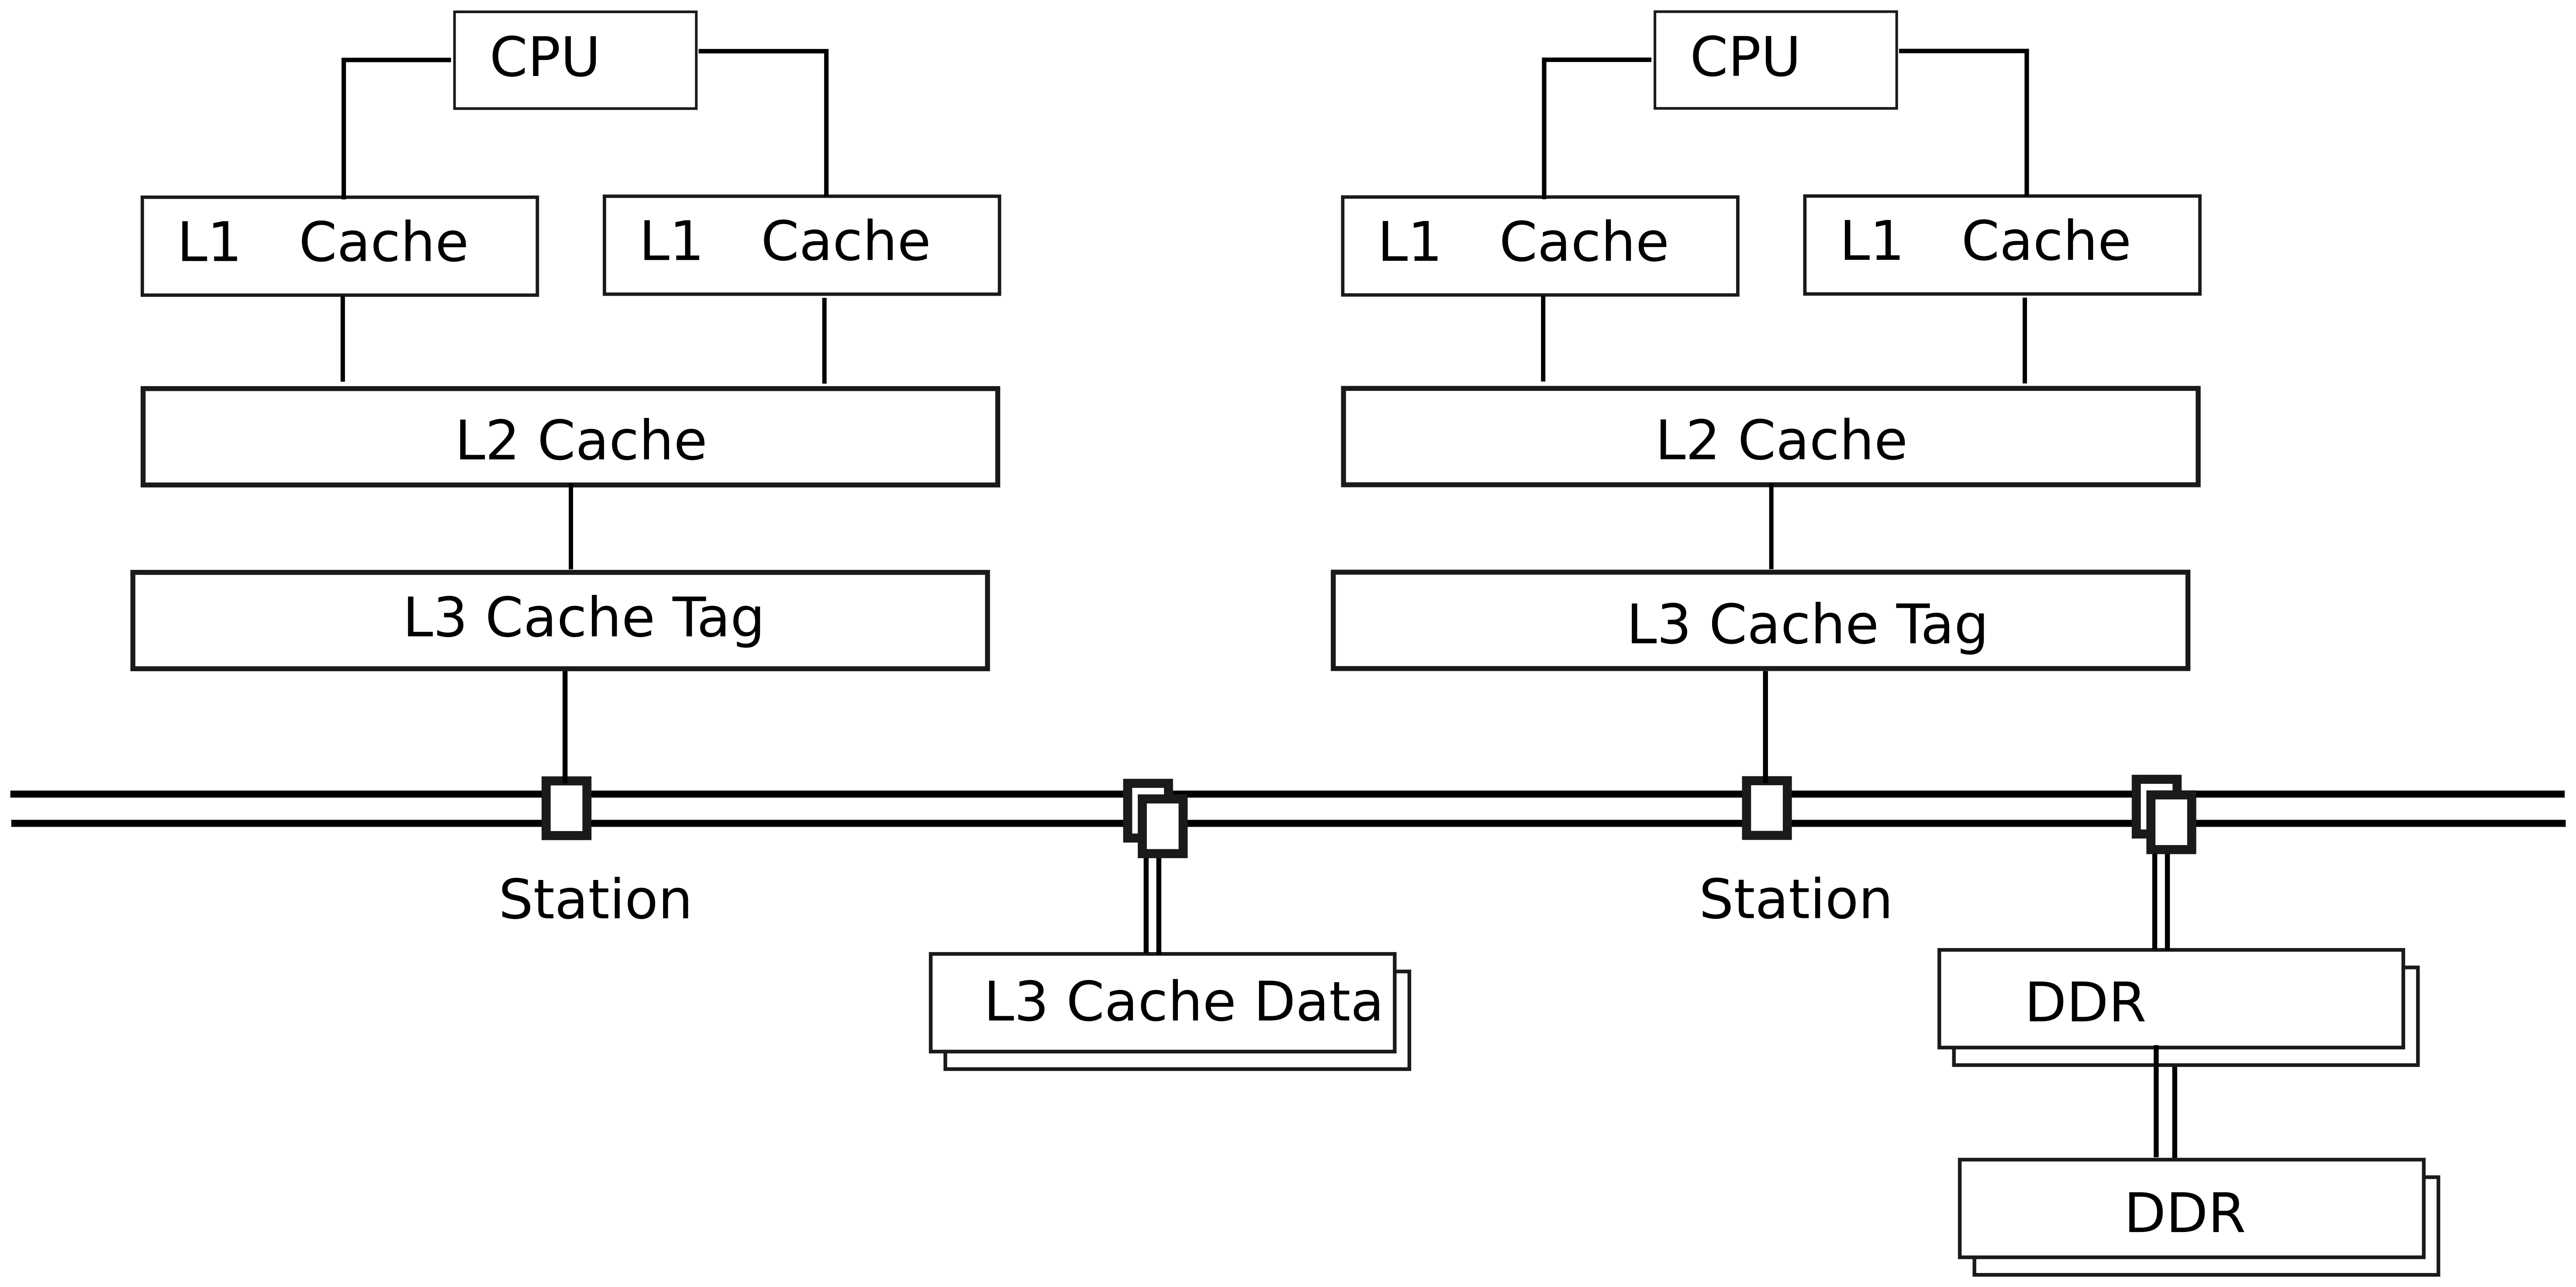
\includegraphics[width=0.7\textwidth]{kp920_cache.png}
    \caption{kunpeng cache示意图}
    \label{Kunpeng Cache示意图}
\end{figure}


Cache在计算机系统中,是一种基于分层优化思想的一种优化手段。由于CPU的速度远大于内存的速度,出于成本的考虑,人们常用相对高速的Cache来弥补两者之间的差距,提升CPU的性能。

图\ref{Kunpeng Cache示意图}为鲲鹏920处理器内存Cache的示意图\cite{kunpeng920pub},在鲲鹏920芯片中,每个核心独占L1、L2两级缓存。离核心最近的是两个L1 Cache,分开缓存指令和数据,大小分别为64K。L2 Cache则要大得多,大小为512k。而第三级缓存则是鲲鹏920芯片上的所有核心共享,其中L3 Cacheline的长度为128个字节。

\subsection{Cache Prefetch}
Cache Prefetch也是一个针对Cache的优化设计。Cache比实际的内存快很多,所以如果我们可以提前加载部分内存到Cache中,就会在性能上有优势。比如一个乘法的时间,就算不考虑流水线,也不过3-12个周期,但是从DDR内存中读取数据可能会花费100个始终周期。所以最好还是在计算开始前,先让数据从内存加载到缓存当中,做到计算和缓存同步进行。

例如,如下代码:
\begin{lstlisting}[language=c++]
    for (i=0; i<W; i++) {
        for(j=0; j<W; j++) {
          c[i][j] = 0;
          if (!(j%INT_PER_CACHELINE))
                  __builtin_prefetch((const void *)&c[i][j+INT_PER_CACHELINE], 1, 3);
          for (k=0; k<H; k++) {
                  c[i][j] += a[i][k]*b[k][j];
                  if (!j && !(k%INT_PER_CACHELINE))
                          __builtin_prefetch((const void *)&a[i][k+INT_PER_CACHELINE], 0, 3);
                  if (!i && !(j%INT_PER_CACHELINE))
                          __builtin_prefetch((const void *)&b[k][j+INT_PER_CACHELINE], 0, 3);
          }
        }
  }
\end{lstlisting}

这里的\_\_builtin\_prefetch是gcc的内置函数,在不同的平台有不同的封装。在上面的算法中,我们进行某个向量单元的计算的时候,已经可以知道后面要计 算的内存单元是什么了,我们就可以提前把数据取出来。除了软件在做prefetch外,鲲鹏920处理器中也有硬件实现的prefetch单元,如\ref{hw_prefetch}。这就导致软件层面的prefetch可以没有很好的效果。

\begin{figure}[htbp]
    \centering
    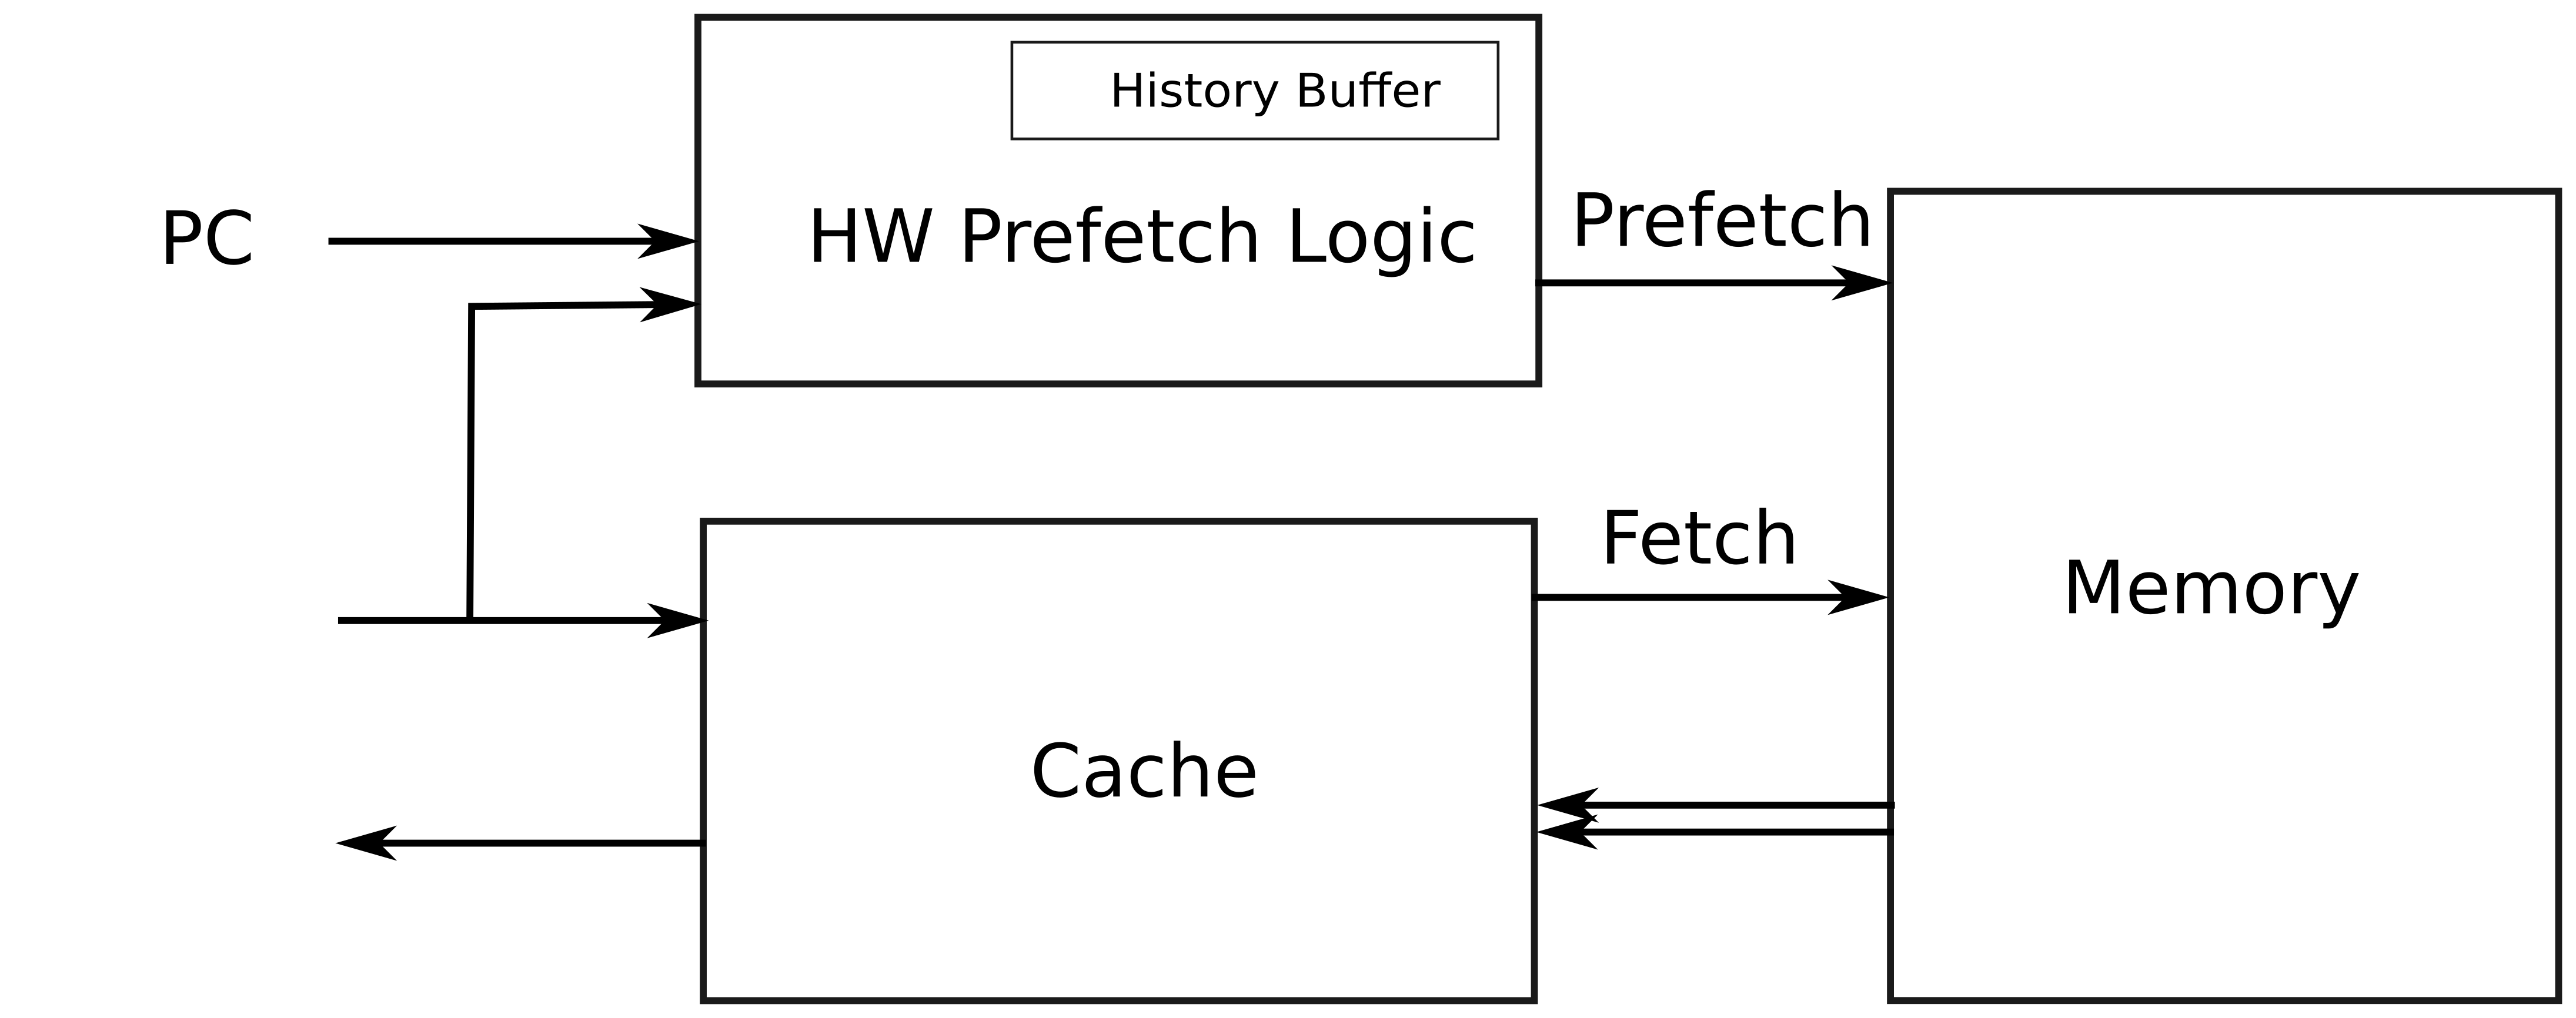
\includegraphics[width=0.7\textwidth]{hw_prefetch.png}
    \caption{鲲鹏920 cache prefetch的硬件结构示意图\cite{kunpeng920pub}}
    \label{hw_prefetch}
\end{figure}

\subsection{缓存一致性协议}

在多核CPU的情况下,由于每个核心都有自己的独占的缓存,数据在这些缓存中制造了多个备份,这就造成了,到底哪份有效的问题。鲲鹏920采用的是监听一致性协议(Snooping),该协议是通过总线广播的形式实现的。最为经典的监听一致性协议是MESI,该协议由 James Goodman 提出,目前已在x86、ARM、Power架构中得到实现。

MESI协议将CacheLine分为四个状态
\begin{enumerate} \setlength{\itemsep}{0pt}
\item Modified(M):该状态表示,此CacheLine有效,数据只存在本cache中,且CacheLine中的数据被修改和内存中的不一样。在这种状态下,如果监听到有其他芯片读取缓存行对应主存的操作,该操作就会被延迟:首先将该操作写回,然后本CacheLine的状态就会变为S。
\item exclusive(E):该状态表示,此CacheLine有效,数据只存在于本cache中,数据和Cache中的数据和对应内存中的数据一致。如果监听到总线中其他线程对该行的读取操作,状态将变为S。
\item Shared(E):该状态表示,此CacheLine有效,数据存在于多个Cache中。如果监听到有其他线程的修改或独享请求,那么改缓存行就变为无效
\item Invalid(I):该状态表示,此CacheLine无效,如果有线程对该数据进行读取,就触发cache miss,重新从内存中读取对应的数据。

\end{enumerate}
此外还有一种基于目录是的MESIF缓存一致性协议,这里就不详细展开,详见\cite{husengseng2017}。

总线本质上是一个去中心化的系统,随着核心数量的增加,维护缓存一致性的成本也会增加。例如,假设32个线程同时在一个变量上做自旋锁的操作,此时如果有一个核心更新了一次spinlock,那么就要通知另外31个线程。如果总线上发生了冲突,会导致计算性能进一步下降。

\subsection{伪共享}
缓存一致性协议以及数据按照CacheLine大小读取到Cache,这两个特点造成了在多核计算中经常出现的问题:伪共享(false sharing)。

\begin{lstlisting}[language=c++]
    #omp parallel for num_threads(10)
    for(int i = 0; i < 10; i++){
        for(int j = 0; j < 10; i++){
            sum[i] += i * j;
        }
    }
\end{lstlisting}

例如上述代码,在鲲鹏920中,CacheLine的大小为128字节,sum数组可能会被分配掉同一个CacheLine中,这种情况下,会导致算法的并行度无法上升。因为一个核心的写操作都会导致其他核心的缓存失效。当其他线程需要读写该区域内存的时候需要首先将修改过的CacheLine写回,然后重新从内存中读取。

通常可以通过padding的方式来解决伪共享的问题,如图\ref{通过padding的方式解决伪共享导致的问题}。对于多线程频繁读写的数据,通过padding,将不想管的数据分配到不同的CacheLine当中。

\begin{figure}[htbp]
    \centering
    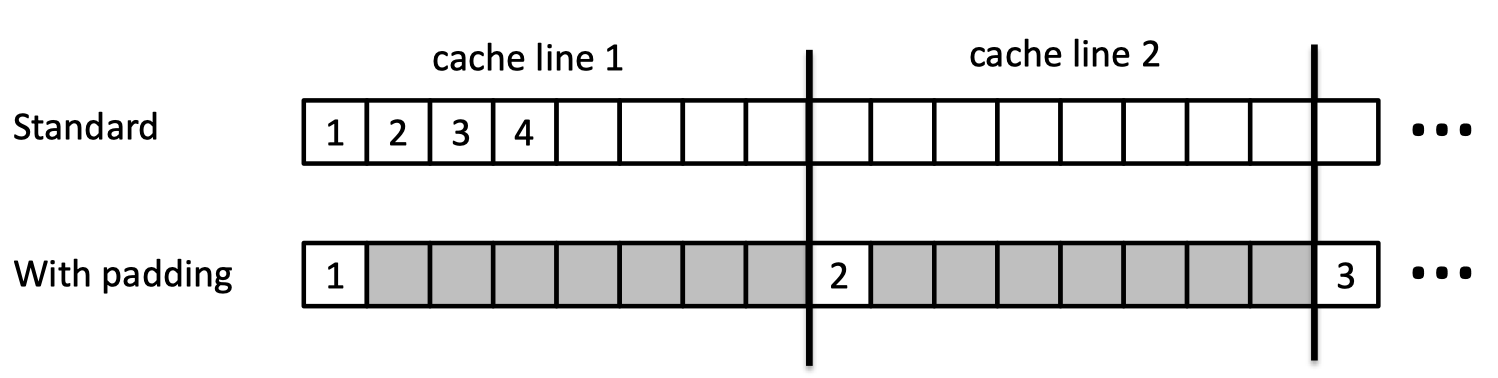
\includegraphics[width=0.7\textwidth]{CacheLine.png}
    \caption{通过padding的方式解决伪共享导致的问题}
    \label{通过padding的方式解决伪共享导致的问题}
\end{figure}

\section{ARM Neon指令}

鲲鹏920处理器基于ARMv8,支持128bits的SIMD指令。它通过在64bits的D寄存器和128bits的Q寄存器上进行向量化的操作,来实现单指令多数据运算。鲲鹏920处理器一共有16个Q寄存器和32个D寄存器。图\ref{SIMD}显示了指令$VADD.I16 Q0, Q1, Q2$同时进行了8路16bit整数的加法操作,相比于传统的加法指令有显著的性能提升。
\begin{figure}[htbp]
    \centering
    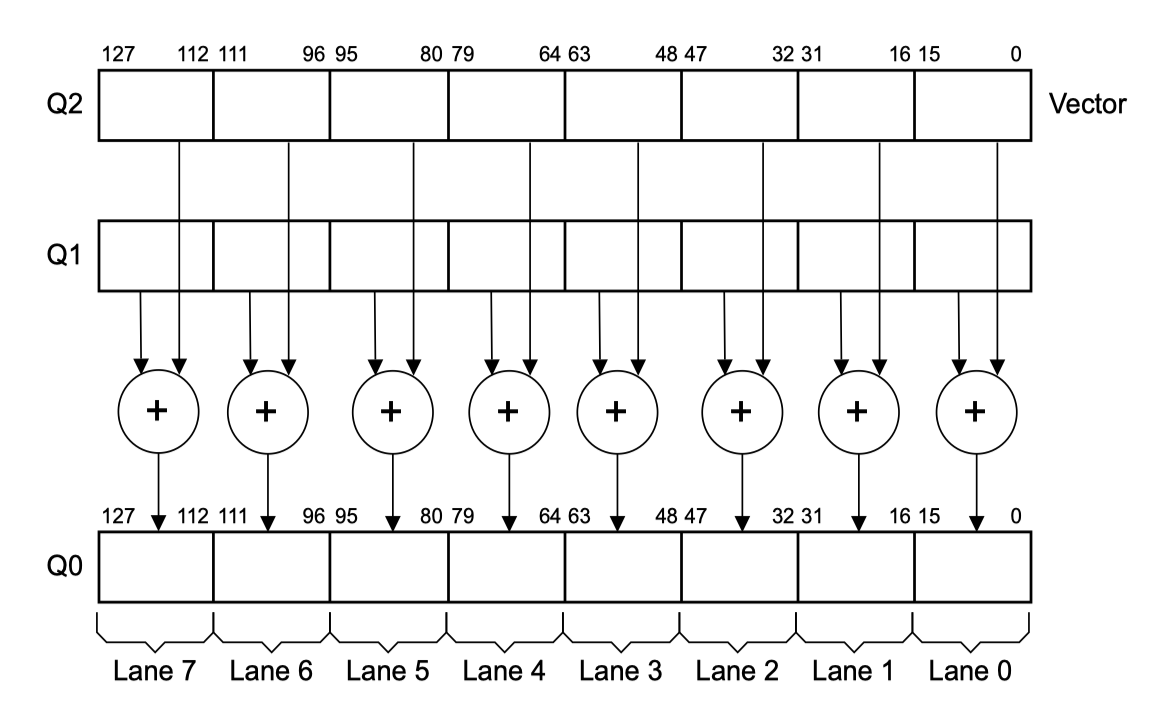
\includegraphics[width=0.7\textwidth]{SIMD.png}
    \caption{8路16位加法操作}
    \label{SIMD}
\end{figure}
ARM Neon除了提供汇编指令之外,还提供了C风格的编程接口Neon intrinsics。相比与Neon汇编指令,使用Neon intrinsics可以不用考虑寄存器的分配问题,这部分由编译器来实现,用户只需要关注上层代码。同时,也能享受编译器带来的一些优化。Neon intrinsics了丰富的编程接口,包括:对数据进行的load与store,各种常用的运算,变量常量的创建等。Neon intrinsics支持GCC编译器,使用时只需include头文件arm\_neon.h。

\section{NUMA架构}

传统多核处理器通常采用SMP(Symmetric Multi-Processing,对称多处理器)\ref{SMP架构示意图},在该架构下,每个线程的地位都是均等的,对内存使用的延迟与带宽也相同。在操作系统的支持下能够做到很好的负载均衡。鲲鹏处理器支持NUMA(Non-uniform memory access, 非统一内存访问)架构,如图\ref{NUMA架构示意图}。使用这种架构能够解决处理器核数限制的问题,同时,通过合理的软件设计,能够提升内存的带宽,解决SMP架构下总线瓶颈的问题。
\begin{figure}[htbp]
    \centering
    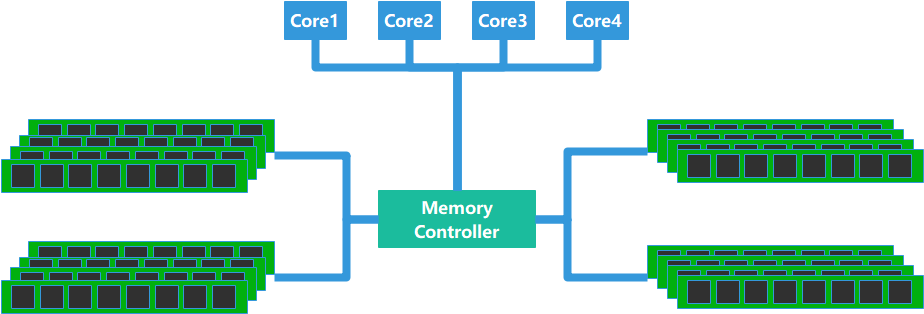
\includegraphics[width=0.7\textwidth]{SMP.png}
    \caption{SMP架构示意图}
    \label{SMP架构示意图}
\end{figure}

由于在NUMA架构下,多个核心组成一个节点(Node),系统中可以存在着多个节点,每个节点上有一个内存控制器,管理控制一片内存。内存在物理上是分布式的,通过片间网络互联。这就导致了,每个线程访问内存的延迟与带宽取决于软件相对于内存的位置,对软件设计者提出了挑战。

\begin{figure}[htbp]
    \centering
    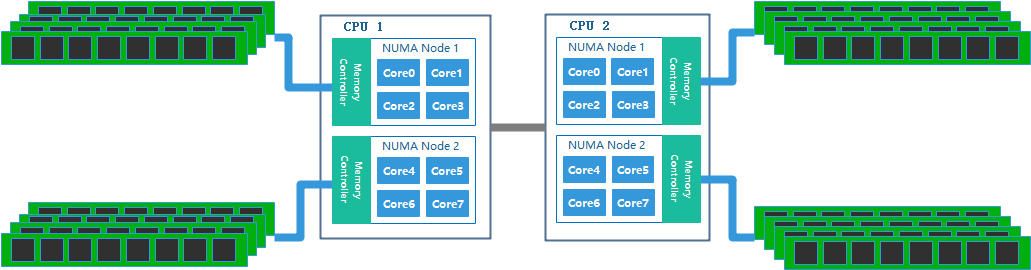
\includegraphics[width=0.7\textwidth]{NUMA.png}
    \caption{NUMA架构示意图}
    \label{NUMA架构示意图}
\end{figure}

linux从内核版本2.5开始就支持NUMA架构\cite{numalinux},用户可以通过numactl命令来手动分配程序的NUMA访问策略,例如我们可以将进程或者内存固定在指定的节点上。系统默认的NUMA策略是nodelocal,及总是在线程执行的地方分配内存。用户可以设置为numactl --interleave,这时操作系统将会在各个节点之间,使用round-robin算法均衡分配内存。同时系统也为用户提供了libnuma这一编程接口\cite{libnuma},方便用户在程序语言层面,对数据进行操作,例如手动指定数据所在的节点。

值得一提的是,默认NUMA策略下,操作系统使用的是“Fist touch”的NUMA分配原则,即用户使用malloc时操作系统会分配逻辑内存页,当初次访问这个数据时(例如初始化操作),操作系统发现该逻辑页面还没有被分配物理页面,于是就进行分配物理页面的操作,此时操作系统的根据调用线程的NUMA分配策略来进行物理页面的分配。这时,在默认NUMA分配政策下,操作系统会将数据分配到,离该线程最接近的NUMA节点。当然也可以开启numactl --interleave,来替换覆盖“First touch”的原则。

常用的编程工具OpenMP也提供了NUMA编程的接口。主要是通过两个环境变量,OMP\_PLACES决定了线程能够创建的位置,可以指定具体的节点,也可指定具体的核心。OMP\_PROC\_BIND可以设置线程的分配方式。

\section{ARMv8原子指令优化}

原子操作是多核程序中一个很重要的操作。x86通常使用锁总线的方式实现原子指令,保证了原子指令的执行期间不会收到其他指令的干扰。

在ARMv8.1发布之前,ARM处理器实现原子操作的方式是ll/sc(Load-Link/Store-Conditional),具体指令就是LDREX/STREX。

具体原理为,当CPU-A调用LOADEX命令的时候,会将数据从内存中读取到缓存当中,并将该缓存的状态标记为EX(Exclusive),此时如果还有一个CPU-B也使用了LOADEX命令,读取同一个数据,这时CPU-B中的标记变成了EX,而CPU-A中缓存行的标记则变成了S。在CPU-A执行完了之后如果要调用STREX指令,将数据写回内存,它首先检查标记的情况,发现自己没了EX,于是写回失败。重新执行LOADEX,操作数据,STREX这样的循环。而CPU-B则可以成功进行STREX,然后放弃EX标记。CPU-A不断处于循环状态,这样就会导致性能的损失。

随着ARM处理器核心数量的提升,原先LL/SC方式的原子操作通过争抢的方式获得原子操作会对性能造成很大的影响。因此,为了支持这种大型系统,在其ARMv8.1规范中引入了LSE (Large System Extensions),加入了大量原生原子操作指令\cite{ArmArchitectureReference},大致原理就是将原子操作放到存储端去做,从而提升多核计算性能,理论上在多核系统的条件下,LSE指令的性能要好与ll/sc原子指令。新的扩展指令包含CAS, SWP和LD/ST<OP>等,其中<op>为ADD,CLR,SET等。

gcc也充分利用了这一特性,提供了基于LSE原子指令的优化。

\begin{lstlisting}[caption={基于LL/SC的原子指令}]
    __LL_SC_PREFIX(arch_atomic_##op(int i, atomic_t *v))			
    {									
        unsigned long tmp;						
        int result;                               
        asm volatile("// atomic_" #op "\n"				
    "	prfm	pstl1strm, %2\n"    
    "1:	ldxr	%w0, %2\n"    
    "	" #asm_op "	%w0, %w0, %w3\n"     				
    "	stxr	%w1, %w0, %2\n"     
    "	cbnz	%w1, 1b"	   
        "=&r" (result), "=&r" (tmp), "+Q" (v->counter)	
        : "Ir" (i));
    }
\end{lstlisting}

\begin{lstlisting}[caption={基于LSE的原子指令}]
    static inline void arch_atomic_##op(int i, atomic_t *v)			
    {									
        register int w0 asm ("w0") = i;					
        register atomic_t *x1 asm ("x1") = v;				
                                        
        asm volatile(ARM64_LSE_ATOMIC_INSN(__LL_SC_ATOMIC(op),		
    "	" #asm_op "	%w[i], %[v]\n")					
        : [i] "+r" (w0), [v] "+Q" (v->counter) 				
        : "r" (x1)   					
        : "x16", "x17", "x30");  					
    }
\end{lstlisting}

对比上述两个不同的实现方式,原来基于LL/SC实现的原子操作,需要先LDXR,然后执行STXR并查看是否成功,如果不成功那就重新循环执行,直到成功。而基于LSE原子指令的实现则更加简洁,如果是atomic\_add操作只需一条LDADD指令。

\section{CPU松弛技术}

在自旋等待中,常常会使用到CPU\_relax()进行优化。也就是在自旋的循环体重插入nop操作,让cpu进行空转。在核并行的情况下,这种操作能够减轻为了维护内存序带来的性能损失。intel处理器从Pentium4开始引入了PAUSE汇编指令。在ARM架构下也能通过汇编实现类似的操作。memory指令是内存屏障的操作,保持CPU空转,在运行时防止对内存的操作乱序执行,并且会将所有缓存在寄存器中的所有变量写回内存当中,然后重新从内存中读取。


\begin{lstlisting}[language=c++]
    inline void PauseCPU() { 
        __asm__ __volatile__("yield" : : : "memory"); 
    }
\end{lstlisting}

\section{本章小结}

本章介绍了SpTRSV算法的应用场景,在线性方程求解算法中,LU分解和预优化的共轭梯度下降法都需要用到稀疏下三角矩阵求解;然后介绍了稀疏矩阵常见的两种几种压缩方式COO、CSC、CSR;之后又详细介绍了目前现有的性能不错的SpTRSV算法及其性能分析。最后介绍了基于多核CPU体系结构进行优化的一些手段,以及这些优化技术的原理。例如缓存优化技术,伪共享的消除机制,基于ARM Neon的SIMD指令,已经针对NUMA架构的优化。最后还提到了使用CPU松弛技术来提高多核并发情况下自旋等待的性能。




\endinput